\documentclass[11pt,a4paper]{article}
\usepackage[a4paper,margin=1.9cm]{geometry}
\usepackage[T1]{fontenc}
\usepackage{lmodern,microtype,amsmath,array,booktabs,graphicx,caption,enumitem,tikz}
\usepackage[colorlinks,linkcolor=black,urlcolor=black,citecolor=black]{hyperref}
\usetikzlibrary{positioning,arrows.meta}
\graphicspath{{../figures/}}
\setlist{nosep,leftmargin=*}
\captionsetup{font=small,labelfont=bf,skip=4pt}
\setlength{\parskip}{3pt}
\setlength{\parindent}{0pt}
\setlength{\textfloatsep}{8pt}

\title{\vspace{-1.4cm}Network Intrusion Detection on UNSW-NB15\\[2pt]
\large Integrated Project, Machine Learning (Prof.\ Youness Moukafih), Subject 13}
\author{Walid El Haimer \and Ayman Ezzougari \and Ahmed Ilyas Elmoussi \and Ahmed Graoui\\[1pt]
\small International University of Rabat, 2026/2027\\
\small Code: \url{https://github.com/naviarok/network-intrusion-detection}\\
\small Its scripts print every number below, unless noted otherwise}
\date{}

\begin{document}
\maketitle
\vspace{-1cm}

%----------------------------------------------------------------------------------------
\section{Task objective}

A network intrusion detection system watches traffic and raises an alarm when a connection looks
malicious. Each sample of the UNSW-NB15 dataset~\cite{unsw} is one \emph{flow} (a connection
between two hosts) described by 42 statistics: duration, bytes and packets in each direction,
time-to-live (TTL) values, load, jitter, connection counters, and three text fields (\texttt{proto},
\texttt{service}, \texttt{state}). We use the official partitions: 175{,}341 training flows and
82{,}332 test flows.\footnote{In the copy we use, the two file names are swapped; the configuration
file corrects this.} The project has two goals:
\begin{enumerate}
\item \textbf{Binary detection:} is a flow normal or an attack (\texttt{label})?
\item \textbf{Attack category:} which of 9 attack types is it (\texttt{attack\_cat}: Generic,
Exploits, Fuzzers, DoS, Reconnaissance, and the rare Analysis, Backdoor, Shellcode, Worms)?
\end{enumerate}
Accuracy alone is not the right goal. Every alarm is checked by a security analyst, so
\textbf{false alarms} (normal flows flagged as attacks) have a real cost. We therefore fix an
operating rule: \emph{at most 5\% of normal traffic may raise an alarm}, and maximise the share of
attacks caught (\emph{detection rate}) under that rule. Following the project guidelines, our focus
is on understanding the data and justifying each preprocessing step with measurements, using simple
models from the course. The final system has two stages (Figure~\ref{fig:system}).

\begin{figure}[h]
\centering
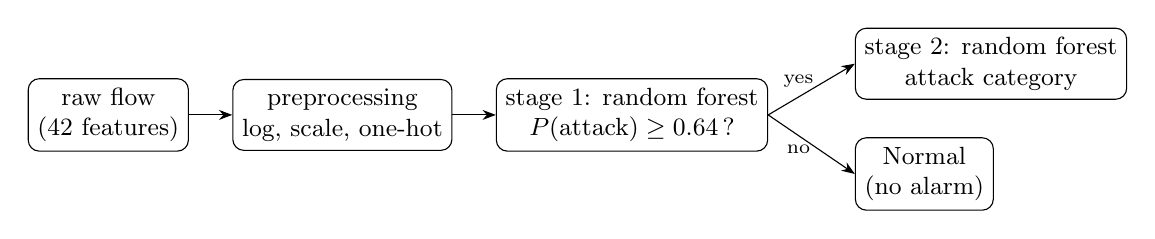
\begin{tikzpicture}[node distance=0.55cm, box/.style={draw, rounded corners, align=center,
  font=\small, minimum height=0.9cm}, >={Stealth}]
\node[box] (in) {raw flow\\(42 features)};
\node[box, right=of in] (prep) {preprocessing\\log, scale, one-hot};
\node[box, right=of prep] (bin) {stage 1: random forest\\$P(\text{attack}) \ge 0.64$\,?};
\node[box, right=1.1cm of bin, yshift=0.65cm] (cat) {stage 2: random forest\\attack category};
\node[box, right=1.1cm of bin, yshift=-0.75cm] (norm) {Normal\\(no alarm)};
\draw[->] (in) -- (prep);
\draw[->] (prep) -- (bin);
\draw[->] (bin.east) -- node[above, font=\scriptsize, pos=0.35] {yes} (cat.west);
\draw[->] (bin.east) -- node[below, font=\scriptsize, pos=0.35] {no} (norm.west);
\end{tikzpicture}
\caption{The two-stage system. Stage 1 decides whether to raise an alarm, with a threshold tuned for
at most 5\% false alarms. Stage 2, trained on attack flows only, names the attack. The two outputs
can therefore never contradict each other.}
\label{fig:system}
\end{figure}

%----------------------------------------------------------------------------------------
\section{Preprocessing pipeline}

\subsection{What the data looks like, and what we decided}
Table~\ref{tab:explore} lists what the exploration (\texttt{explore.py}) revealed and the decision
each finding led to.

\begin{table}[h]
\centering\small
\begin{tabular}{p{0.47\linewidth}p{0.47\linewidth}}
\toprule
Finding & Decision \\
\midrule
No missing values in either file. & No imputation needed. \\
\textbf{38.6\%} of the training rows (67{,}601) repeat another row exactly. Generic drops from
40{,}000 to 4{,}181 rows, DoS from 12{,}264 to 3{,}806. &
Remove duplicates \emph{before} splitting, otherwise copies land on both sides of the
train/validation split (measured in Table~\ref{tab:study}B). \\
1{,}772 identical flows carry 2+ attack categories; 229 are both normal and attack. &
Nothing to fix: this is an error floor that no model can beat (Section~\ref{sec:multi}). \\
Counts are extremely skewed: \texttt{sbytes} has median 430 and maximum $1.3\times10^{7}$;
\texttt{sload} reaches $6\times10^{9}$. All values are $\ge 0$. &
Apply $\log(1+x)$ to every numeric feature, then standardise (mean 0, standard deviation 1). \\
Features have unrelated units (seconds, bytes, flags). & Standardisation, needed by logistic
regression and KNN (measured in Table~\ref{tab:study}A). \\
3 text columns; \texttt{proto} has 133 values, many very rare; \texttt{state} values ACC and CLO
appear only in the test file. &
One-hot encoding; values seen fewer than 100 times share one ``infrequent'' column, which also
receives values never seen in training. \\
Strong imbalance: 51{,}890 normal vs.\ 127 Worms flows after de-duplication. &
Stratified split; macro F1 for model selection; \texttt{class\_weight} in the search space. \\
Source TTL almost gives the answer away: TTL 31 is 0\% attacks, TTL 254 is 90.2\%. &
Kept, but checked as a possible artefact of the testbed (Table~\ref{tab:study}C). \\
\bottomrule
\end{tabular}
\caption{Exploration findings (training file) and the preprocessing decision each one led to.}
\label{tab:explore}
\end{table}

\textbf{Pipeline and data splits.} After de-duplication, the 107{,}740 training rows are split 80/20
into \emph{train} (86{,}192) and \emph{validation} (21{,}548), stratified by attack category so that
even Worms appears in both. All hyperparameters and the alarm threshold are chosen on validation.
The official test file is only opened by \texttt{test.py}, after training. The transformations are
wrapped with the classifier in one scikit-learn \texttt{Pipeline}, so means, standard deviations and
category lists are learned on the train rows only (no leakage), and the saved model accepts raw flows
directly.

\subsection{Does each choice matter? Measured effect}
\texttt{preprocessing\_study.py} changes one choice at a time and keeps fixed models from the course
(Table~\ref{tab:study}). Score: detection rate on validation when the threshold allows at most 5\%
false alarms.

\begin{table}[h]
\centering\small
\begin{tabular}{llccc}
\toprule
\multicolumn{5}{l}{\textbf{A. Numeric scaling} (validation)} \\
Model & Scaling & Detection @5\% FA & ROC AUC & Macro F1, categories \\
\midrule
Logistic regression ($C{=}1$) & none$^{*}$ & 0.209 & 0.828 & 0.182 \\
 & standard & 0.775 & 0.968 & 0.381 \\
 & \textbf{log + standard} & \textbf{0.814} & \textbf{0.974} & \textbf{0.425} \\
KNN ($k{=}5$) & none$^{\dagger}$ & 0.000 & 0.885 & 0.294 \\
 & standard & 0.707 & 0.964 & 0.442 \\
 & \textbf{log + standard} & \textbf{0.865} & \textbf{0.973} & \textbf{0.495} \\
Decision tree (depth 10) & none & 0.870 & 0.979 & 0.597 \\
 & standard & 0.865 & 0.979 & 0.594 \\
 & log + standard & 0.870 & 0.979 & 0.597 \\
\midrule
\multicolumn{5}{l}{\textbf{B. Duplicate rows} (the test file is shown only as an after-the-fact check)} \\
Model & Duplicates & Val detection & Test detection & Test false alarms \\
\midrule
Logistic regression & removed & 0.814 & 0.906 & 0.136 \\
 & kept & 0.909 & 0.912 & 0.144 \\
Random forest & removed & 0.908 & 0.964 & 0.168 \\
 & kept & 0.958 & 0.970 & 0.182 \\
\midrule
\multicolumn{5}{l}{\textbf{C. TTL features} \texttt{sttl, dttl, ct\_state\_ttl}} \\
Model & TTL & Val detection & Test detection & Test false alarms \\
\midrule
Logistic regression & kept & 0.814 & 0.906 & 0.136 \\
 & dropped & 0.668 & 0.804 & 0.144 \\
Random forest & kept & 0.908 & 0.964 & 0.168 \\
 & dropped & 0.902 & 0.958 & 0.162 \\
\bottomrule
\end{tabular}
\caption{Effect of each preprocessing choice. FA = false alarms, Val = validation. $^{*}$did not converge in 2{,}000 iterations. $^{\dagger}$no threshold reaches 5\% false alarms.}
\label{tab:study}
\end{table}

\textbf{What we learn.}
(A)~Scaling is decisive for the distance- and gradient-based models and irrelevant for trees, exactly
as the course predicts. A tree only compares one feature with a cut-off, and any increasing transform
keeps the same order. Without scaling, logistic regression does not converge in 2{,}000 iterations,
and KNN distances are dominated by the byte counts: its probabilities (multiples of $1/5$) cannot get
the false alarm rate under 5\%. The log step adds a further $+4$ points (logistic regression) and
$+16$ points (KNN) over plain standardisation, because it stops a few huge flows from dominating.
(B)~Keeping the duplicates makes validation look 5--10 points better, but test detection barely moves
and false alarms get worse. The extra validation score was copies being recognised, not real
learning. (C)~The TTL features carry real signal for the linear model ($-15$ points without them),
while the forest finds the same information elsewhere. Dropping them does \emph{not} fix the false
alarms on the test file (Section~\ref{sec:fa}), so we keep them.

%----------------------------------------------------------------------------------------
\section{Models and hyperparameters}

We compare three classifiers from the course: \textbf{logistic regression} (a linear score passed
through a sigmoid, the interpretable baseline), a \textbf{decision tree} (yes/no questions,
nonlinear, needs no scaling) and a \textbf{random forest} (bagged trees on random feature subsets,
which lowers the variance of a deep tree). KNN is used only in the preprocessing study: it must keep
all 86{,}192 training rows and compare every new flow with each of them, which is too slow for a
detector. The search space (in \texttt{configs/config.yaml}) is a full grid; every combination is
trained on train and scored on validation:

\begin{center}\small
\begin{tabular}{>{\raggedright\arraybackslash}p{0.19\linewidth}>{\raggedright\arraybackslash}p{0.33\linewidth}>{\raggedright\arraybackslash}p{0.4\linewidth}}
\toprule
Model & Stage 1: normal vs.\ attack & Stage 2: attack category \\
\midrule
Logistic regression & $C \in \{0.01, 0.1, 1, 10\}$ & $C \in \{0.1, 1, 10\}$; class\_weight $\in$ \{none, balanced\} \\
Decision tree & max\_depth $\in \{5,10,20,\infty\}$; min\_leaf $\in\{1,10\}$ & max\_depth $\in\{10,20,\infty\}$; min\_leaf $\in\{1,10\}$; class\_weight $\in$ \{none, balanced\} \\
Random forest (100 trees) & max\_depth $\in\{10,20\}$; min\_leaf $\in\{1,5\}$ & max\_depth 20; min\_leaf $\in\{1,5\}$; class\_weight $\in$ \{none, balanced\_subsample\} \\
\midrule
Selection score & detection rate at $\le$5\% false alarms & macro F1 (each category counts equally) \\
\bottomrule
\end{tabular}
\end{center}

For stage 1, each candidate gets its own threshold: the lowest $t$ (in steps of 0.01) such that at
most 5\% of normal validation flows have $P(\text{attack}) \ge t$. Candidates that cannot meet the
rule get a score of 0. This rule matters in practice: the leaves of a fully grown tree are pure, so
almost all its probabilities are exactly 0 or 1. Even a threshold of 1.0 then flags more than 5\% of
normal flows, so the tree is rejected, even though its raw alarms catch many attacks. Stage 2 is trained on attack flows only. Macro F1
is the plain average of the per-category F1 scores, so Worms (127 rows) weighs as much as Exploits.

\textbf{Search results (validation).} Stage 1: random forest, max\_depth 20, min\_leaf 1:
detection \textbf{0.908} at threshold \textbf{0.64} (ROC AUC 0.987), ahead of the best tree (0.878)
and logistic regression (0.825, $C{=}10$). Stage 2: random forest, max\_depth 20, min\_leaf 5,
class\_weight = balanced\_subsample: macro F1 \textbf{0.602}, closely followed by a depth-10 tree
(0.597), with logistic regression far behind (0.445). Class weighting helped the forest by
$+0.07$ macro F1, for almost the same accuracy (0.762 vs.\ 0.763): it trades errors on large classes for
recall on rare ones. A forest takes about 5\,s to train, logistic regression up to 25\,s (stage 2).

%----------------------------------------------------------------------------------------
\section{Evaluation and results}

\textbf{Methodology.} The saved models are evaluated once, by \texttt{test.py}, on the 82{,}332 flows
of the official test file, which played no part in any choice. We report the detection rate (recall
on attacks), precision (share of alarms that are real attacks), false alarm rate (share of normal
flows flagged), F1 and ROC AUC for stage 1; per-category precision, recall and F1 for stage 2.

\subsection{Stage 1: detection}
\begin{center}\small
\begin{tabular}{lcccccc}
\toprule
Test set & Accuracy & Detection rate & Precision & False alarm rate & F1 & ROC AUC \\
\midrule
threshold 0.5 & 0.870 & 0.987 & 0.816 & 0.273 & 0.893 & 0.983 \\
threshold 0.64 (chosen) & \textbf{0.905} & 0.964 & \textbf{0.875} & \textbf{0.168} & \textbf{0.918} & 0.983 \\
\bottomrule
\end{tabular}
\end{center}

\begin{figure}[h]
\centering
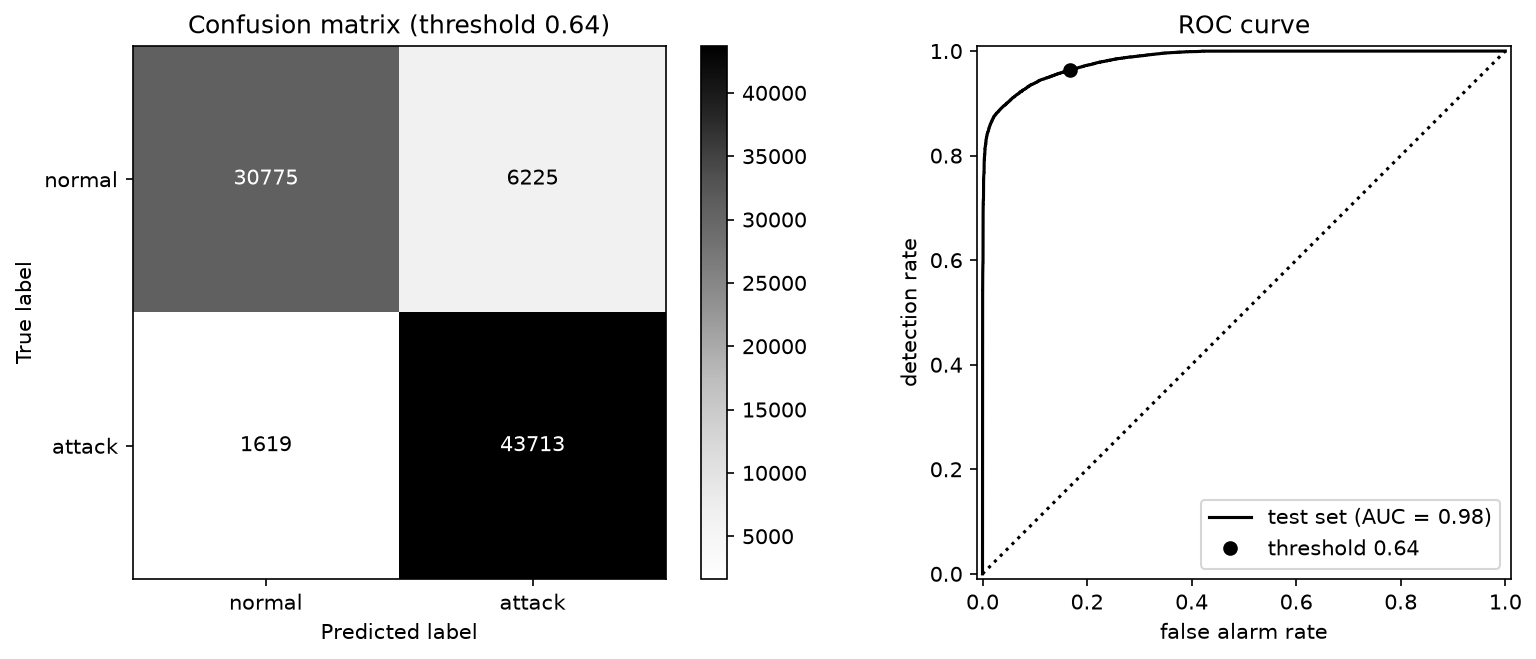
\includegraphics[width=0.82\linewidth]{test_confusion_roc.png}
\caption{Test set, stage 1. Left: 6{,}225 false alarms and 1{,}619 missed attacks out of 82{,}332
flows. Right: ROC curve; the dot is the chosen operating point.}
\label{fig:roc}
\end{figure}

The tuned threshold removes 38\% of the false alarms of the default 0.5 (27.3\% $\to$ 16.8\%) for
2.3 points of detection. Almost every attack type is caught: Generic 100\%, DoS 99.8\%,
Reconnaissance 99.8\%, Backdoor 99.8\%, Exploits 99.0\%, Shellcode 98.7\%, Worms 97.7\% (43 of 44),
Analysis 97.3\%. The exception is \textbf{Fuzzers} (75.8\%). Fuzzers send random, malformed traffic
that partly resembles normal traffic.

\subsection{Investigating false alarms}\label{sec:fa}
The main issue is that the false alarm rate is \textbf{16.8\% on test instead of the 5\% chosen on
validation}. Grouping the 37{,}000 normal test flows reveals where the alarms come from. Normal flows
with source TTL 31 (16{,}702 flows) never raise an alarm, those with TTL 62 do in 11.8\% of cases, and
those with TTL 254 in \textbf{38.1\%}. In the training file, TTL 254 means an attack 90\% of the time.
The test file contains many more normal flows of exactly this kind:

\begin{center}\small
\begin{tabular}{lcccc}
\toprule
Source TTL of normal flows & 0 & 31 & 62 & 254 \\
\midrule
share in the training file & 5.1\% & 70.5\% & 3.9\% & 20.1\% \\
share in the test file & 2.7\% & 45.1\% & 11.2\% & \textbf{40.7\%} \\
\bottomrule
\end{tabular}
\end{center}

By service, false alarms concentrate on flows without an identified service (``-'', 19.8\%), FTP
(26.6\%) and HTTP (15.2\%), while DNS, SMTP and SSH have none. So the normal traffic of the test file
is \emph{distributed differently} from the normal traffic the threshold was calibrated on: a
\emph{distribution shift}. Validation could not reveal it, because it comes from the training file.
Table~\ref{tab:study}C shows that removing the TTL features does not solve it (16.2\% false alarms),
so the shift affects more than these columns. In deployment, the threshold would have to be
re-calibrated on recent normal traffic of the protected network.

\subsection{Stage 2: attack categories and rare classes}\label{sec:multi}
\begin{center}\small
\begin{tabular}{lccccccccc|c}
\toprule
Test attacks & Gen. & Expl. & Fuzz. & DoS & Recon. & Anal. & Backd. & Shell. & Worms & macro \\
\midrule
flows & 18{,}871 & 11{,}132 & 6{,}062 & 4{,}089 & 3{,}496 & 677 & 583 & 378 & 44 & \\
precision & 0.998 & 0.848 & 0.825 & 0.570 & 0.869 & 0.072 & 0.056 & 0.269 & 0.517 & 0.558 \\
recall & 0.971 & 0.608 & 0.720 & 0.120 & 0.839 & 0.257 & 0.544 & 0.926 & 0.705 & 0.632 \\
F1 & 0.984 & 0.708 & 0.769 & 0.198 & 0.853 & 0.112 & 0.101 & 0.417 & 0.596 & 0.526 \\
\bottomrule
\end{tabular}
\end{center}

\begin{figure}[h]
\centering
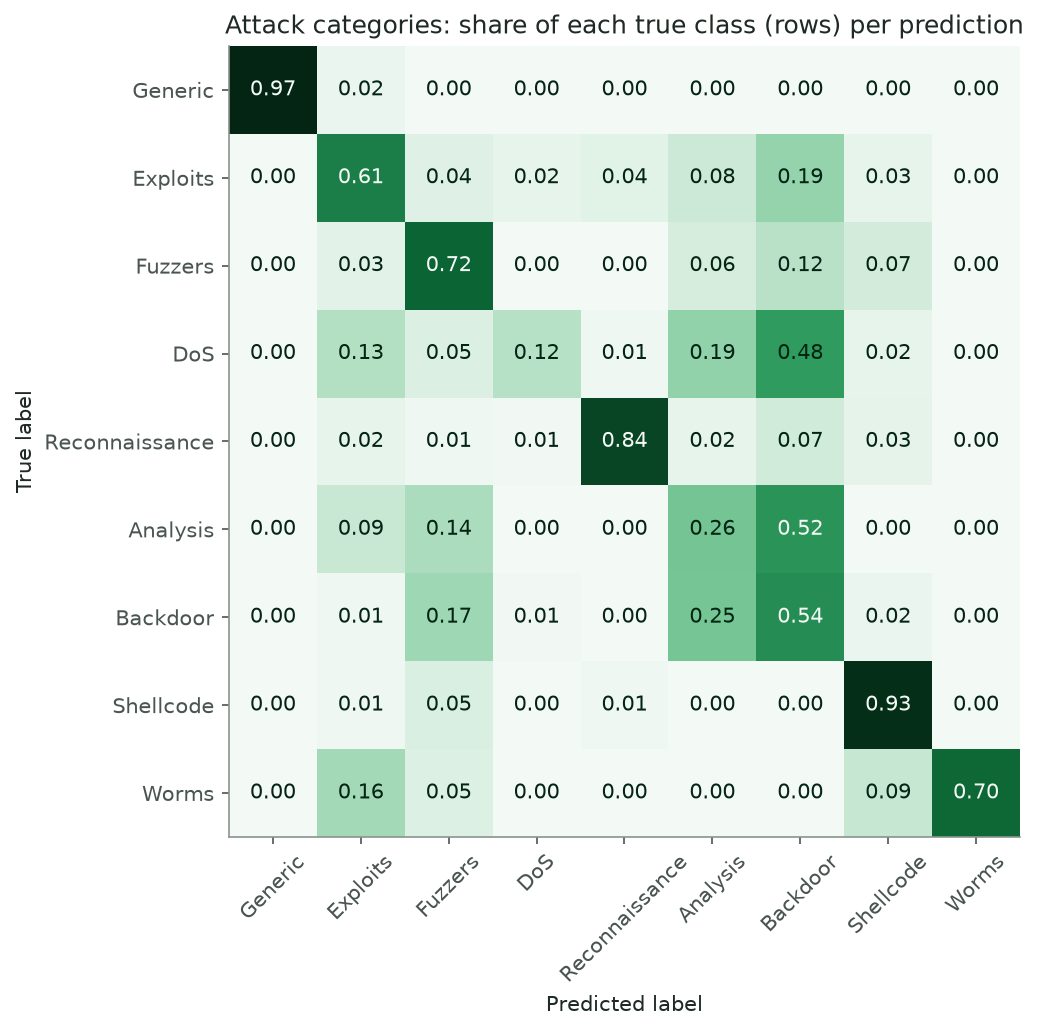
\includegraphics[width=0.5\linewidth]{test_multiclass_confusion.png}
\caption{Stage 2 on the 45{,}332 test attacks. Rows: true category; each row sums to 1, and the
diagonal is the recall.}
\label{fig:multi}
\end{figure}

Generic, Reconnaissance and Shellcode are well separated, and even \textbf{Worms}, with only 127
training flows, is recognised 70.5\% of the time. The weak spot is the group \textbf{DoS / Analysis /
Backdoor / Exploits} (Figure~\ref{fig:multi}). 48\% of DoS flows are predicted as Backdoor, and half
of Analysis as well. These categories share the same flow statistics: this is where the training
file contains identical flows with different categories (Table~\ref{tab:explore}). The class
weighting pushes these ambiguous flows towards the small classes, which explains the very low
precision of Analysis (0.072) and Backdoor (0.056): they are predicted often, but mostly for DoS or
Exploits flows. Macro F1 drops from 0.602 on validation to 0.526 on test, again a sign of the shift
between the two files.

\textbf{Complete system} (stage 1, then stage 2, on all 82{,}332 test flows, 10 classes): macro F1
0.509, support-weighted F1 0.796, Normal recall 0.832. An earlier version of our code used a single
10-class forest trained on all flows instead. It scored lower (macro F1 0.489) and contradicted the
detector, labelling 41\% of normal test flows as attacks. That is why we moved to two stages.

%----------------------------------------------------------------------------------------
\section{Limitations and future work}
\begin{itemize}
\item \textbf{Distribution shift} is the main limitation: a threshold that guarantees 5\% false
alarms on validation gives 16.8\% on test. Remedies: re-calibrate the threshold on recent normal
traffic, monitor the false alarm rate in operation, or validate on data closer to deployment
(for example a time-ordered split, if timestamps were available).
\item \textbf{Ambiguous categories.} DoS, Analysis, Backdoor and Exploits overlap in feature space,
so no classifier on these 42 statistics can separate them reliably. Options: merge them into one
category, use payload or packet-level features, or report the top-2 categories to the analyst.
\item \textbf{Rare classes:} 127 Worms flows are few; class weights help recall but hurt precision.
Resampling (e.g.\ oversampling the minority classes) inside the training folds could be compared.
\item \textbf{Evaluation:} one stratified validation split; $k$-fold cross-validation would give
error bars on every number. The search grid is small and could be extended (e.g.\ number of trees,
\texttt{max\_features}).
\item \textbf{Models:} gradient boosting and AdaBoost (also in the course) could add accuracy.
Logistic regression stays useful as an interpretable baseline: its weights show which features
push towards an alarm.
\end{itemize}

\begin{thebibliography}{1}\small
\bibitem{unsw} N.~Moustafa and J.~Slay, ``UNSW-NB15: a comprehensive data set for network intrusion
detection systems (UNSW-NB15 network data set)'', \emph{Military Communications and Information
Systems Conference (MilCIS)}, 2015.
\end{thebibliography}

\end{document}
